\newif\ifshowsolutions
\showsolutionstrue
\documentclass{article}
\usepackage{listings}
\usepackage{xcolor}
\usepackage{amsmath}

% Python syntax highlighting colors
\definecolor{codegreen}{rgb}{0,0.6,0}
\definecolor{codegray}{rgb}{0.5,0.5,0.5}
\definecolor{codepurple}{rgb}{0.58,0,0.82}
\definecolor{codeblue}{rgb}{0.0,0.0,0.8}
\definecolor{codeorange}{rgb}{0.8,0.4,0.0}
\definecolor{backcolour}{rgb}{0.97,0.97,0.97}

% Python listings style
\lstdefinestyle{pythonstyle}{
    backgroundcolor=\color{backcolour},
    commentstyle=\color{codegreen},
    keywordstyle=\color{codeblue}\bfseries,
    numberstyle=\tiny\color{codegray},
    stringstyle=\color{codeorange},
    basicstyle=\ttfamily\footnotesize,
    breakatwhitespace=false,
    breaklines=true,
    captionpos=b,
    keepspaces=true,
    numbers=left,
    numbersep=5pt,
    showspaces=false,
    showstringspaces=false,
    showtabs=false,
    tabsize=4,
    frame=single,
    framerule=0.5pt,
    rulecolor=\color{codegray},
}

\lstset{style=pythonstyle}
\usepackage{subfig}
\usepackage{amsthm}
\usepackage{amsmath}
\usepackage{amssymb}
\usepackage{graphicx}
\usepackage{mdwlist}
\usepackage{geometry}
\usepackage{titlesec}
\usepackage{palatino}
\usepackage{mathrsfs}
\usepackage{fancyhdr}
\usepackage{paralist}
\usepackage{todonotes}
\usepackage{tikz}
\usepackage{float} % Place figures where you ACTUALLY want it
\usepackage{comment} % A hack to toggle sections
\usepackage{ifthen}
\usepackage{mdframed}
\usepackage{verbatim}
\usepackage{listings}
\usepackage{bbm}
\usepackage{upquote} % Prevents backticks replacing single-quotes in verbatim
\usepackage[strings]{underscore}
\usepackage[colorlinks=true]{hyperref}
\usetikzlibrary{positioning,shapes,backgrounds}

\geometry{margin=1in}
\geometry{headheight=2in}
\geometry{top=2in}

\setlength{\marginparwidth}{2.15cm}
\setlength{\parindent}{0em}
\setlength{\parskip}{0.6\baselineskip}

\rhead{}
\lhead{}

% Spacing settings.
\titlespacing\section{0pt}{12pt plus 2pt minus 2pt}{0pt plus 2pt minus 2pt}
\titlespacing\subsection{0pt}{12pt plus 4pt minus 2pt}{0pt plus 2pt minus 2pt}
\titlespacing\subsubsection{0pt}{12pt plus 4pt minus 2pt}{0pt plus 2pt minus 2pt}
\renewcommand{\baselinestretch}{1.15}

% Shortcuts for commonly used operators.
\newcommand{\E}{\mathbb{E}}
\newcommand{\Var}{\operatorname{Var}}
\newcommand{\Cov}{\operatorname{Cov}}
\newcommand{\Bias}{\operatorname{Bias}}
\DeclareMathOperator{\argmin}{arg\,min}
\DeclareMathOperator{\argmax}{arg\,max}

% Do not number subsections and below.
\setcounter{secnumdepth}{1}

% Custom format subsection.
\titleformat*{\subsection}{\large\bfseries}

% Set up the problem environment.
\newcounter{problem}[section]
\newenvironment{problem}[1][]
  {\begingroup
    \setlength{\parskip}{0em}
    \refstepcounter{problem}\par\addvspace{1em}\textbf{Problem~\Alph{problem}\!
    \ifthenelse{\equal{#1}{}}{}{ [#1 points]}:}
  \endgroup}

% Set up the subproblem environment.
\newcounter{subproblem}[problem]
\newenvironment{subproblem}[1][]
  {\begingroup
    \setlength{\parskip}{0em}
    \refstepcounter{subproblem}\par\medskip\textbf{\roman{subproblem}.\!
    \ifthenelse{\equal{#1}{}}{}{ [#1 points]:}}
  \endgroup}

% Set up the problem command (standalone version).
\providecommand{\problem}[1][]{\refstepcounter{problem}\par\addvspace{1em}\textbf{Problem~\Alph{problem}\ifthenelse{\equal{#1}{}}{}{ [#1 points]}:}}

% Set up the teachers and materials commands.
\newcommand\teachers[1]
  {\begingroup
    \setlength{\parskip}{0em}
    \vspace{0.3em} \textit{\hspace*{2em} TAs responsible: #1} \par
  \endgroup}
\newcommand\materials[1]
  {\begingroup
    \setlength{\parskip}{0em}
    \textit{\hspace*{2em} Relevant materials: #1} \par \vspace{1em}
  \endgroup}

% Set up the hint environment.
\newenvironment{hint}[1][]
  {\begin{em}\textbf{Hint: }}
  {\end{em}}


% Set up the solution environment.
\ifshowsolutions
  \newenvironment{solution}[1][]
    {\par\medskip \begin{mdframed}\textbf{Solution~\Alph{problem}#1:} \begin{em}}
    {\end{em}\medskip\end{mdframed}\medskip}
  \newenvironment{subsolution}[1][]
    {\par\medskip \begin{mdframed}\textbf{Solution~\Alph{problem}#1.\roman{subproblem}:} \begin{em}}
    {\end{em}\medskip\end{mdframed}\medskip}
\else
  \excludecomment{solution}
  \excludecomment{subsolution}
\fi




%%%%%%%%%%%%%%%%%%%%%%%%%%%%%%
% HEADER
%%%%%%%%%%%%%%%%%%%%%%%%%%%%%%

\chead{
  {\vbox{
      \vspace{2mm}
      \large
      Machine Learning \& Data Mining \hfill
      Caltech CS/CNS/EE 155 \hfill \\[1pt]
      Set 4\hfill
      January 27 2026. \\
    }
  }
}

\begin{document}
\pagestyle{fancy}



%%%%%%%%%%%%%%%%%%%%%%%%%%%%%%
% PROBLEM 1
%%%%%%%%%%%%%%%%%%%%%%%%%%%%%%

\newpage
\section{My code}
My solutions and code are in   \href{https://drive.google.com/drive/folders/100BU9aX5GGRsIe0h5_QuuEcg0FLf8EC_?usp=sharing}{the next link}
\section{Deep Learning Principles [35 Points]}
\materials{lectures on deep learning}

For problems A and B, we'll be utilizing the \href{http://playground.tensorflow.org/}{Tensorflow Playground} to visualize/fit a neural network.

\begin{problem}[5]
  Backpropagation and Weight Initialization Part 1
\end{problem}

Fit the neural network at \href{http://playground.tensorflow.org/#activation=relu&batchSize=10&dataset=circle&regDataset=reg-plane&learningRate=0.03&regularizationRate=0&noise=0&networkShape=4,2&seed=0.65409&showTestData=false&discretize=false&percTrainData=50&x=true&y=true&xTimesY=false&xSquared=false&ySquared=false&cosX=false&sinX=false&cosY=false&sinY=false&collectStats=false&problem=classification&initZero=false&hideText=false}{this link} for about 250 iterations, and then do the same for the neural network at  \href{http://playground.tensorflow.org/#activation=relu&batchSize=10&dataset=circle&regDataset=reg-plane&learningRate=0.03&regularizationRate=0&noise=0&networkShape=4,2&seed=0.6&showTestData=false&discretize=false&percTrainData=50&x=true&y=true&xTimesY=false&xSquared=false&ySquared=false&cosX=false&sinX=false&cosY=false&sinY=false&collectStats=false&problem=classification&initZero=true&hideText=false}{this link}.  Both networks have the same architecture and use ReLU activations.  The only difference between the two is how the layer weights were initialized -- you can examine the layer weights by hovering over the edges between neurons.

Give a mathematical justification, based on what you know about the backpropagation algorithm and the ReLU function, for the difference in the performance of the two networks.

\begin{subsolution}

\end{subsolution}

\newpage

\begin{problem}[5]
  Backpropagation and Weight Initialization Part 2
\end{problem}

Reset the two demos from part i (there is a reset button to the left of the ``Run'' button), change the activation functions of the neurons to sigmoid instead of ReLU, and train each of them for 4000 iterations.

Explain the differences in the models learned, and the speed at which they were learned, from those of part i in terms of the backpropagation algorithm and the sigmoid function.

\begin{subsolution}

\end{subsolution}

\newpage


\problem \textbf{[10 Points]}

When training any model using SGD, it's important to shuffle your data to avoid correlated samples. To illustrate one reason for this that is particularly important for ReLU networks, consider a dataset of 1000 points, 500 of which have positive (+1) labels, and 500 of which have negative (-1) labels. What happens if we train a fully-connected network with ReLU activations using SGD, looping through all the negative examples before any of the positive examples? (Hint: this is called the ``dying ReLU'' problem.)


\begin{solution}

\end{solution}

\newpage



\problem Approximating Functions Part 1 \textbf{[7 Points]}

Draw or describe a fully-connected network with ReLU units that implements the OR function on two 0/1-valued inputs,  $x_1$ and $x_2$.  Your networks should contain the minimum number of hidden units possible.  The OR function $\text{OR}(x_1, x_2)$ is defined as:
\begin{gather*}
\text{OR}(1, 0) \geq 1 \\
\text{OR}(0, 1) \geq 1 \\
\text{OR}(1, 1) \geq 1 \\
\text{OR}(0, 0) = 0
\end{gather*}

Your network need only produce the correct output when $x_1 \in \{0, 1\}$ and $x_2 \in \{0, 1\}$ (as described in the examples above).

\begin{subsolution}

\end{subsolution}

\newpage


\problem Approximating Functions Part 2 \textbf{[8 Points]}

What is the minimum number of fully-connected layers (with ReLU units) needed to implement an XOR of two 0/1-valued inputs $x_1, x_2$? Recall that the XOR function is defined as:
\begin{gather*}
\text{XOR}(1, 0) \geq 1 \\
\text{XOR}(0, 1) \geq 1 \\
\text{XOR}(0, 0) = \text{XOR}(1, 1) = 0
\end{gather*}

For the purposes of this problem, we say that a network $f$ computes the XOR function if $f(x_1, x_2) = \text{XOR}(x_1, x_2)$ when $x_1 \in \{0, 1\}$ and $x_2 \in \{0, 1\}$ (as described in the examples above).

Explain why a network with fewer layers than the number you specified cannot compute XOR.

\begin{subsolution}

\end{subsolution}


% problem 2
\newpage
\section{Depth vs Width on the MNIST Dataset  [25 Points]}

MNIST is a classic dataset in computer vision. It consists of images of handwritten digits (0 - 9) and the correct digit classification. In this problem you will implement a deep network using PyTorch to classify MNIST digits. Specifically, you will explore what it really means for a network to be "deep", and how depth vs. width impacts the classification accuracy of a model. You will be allowed at most $N$ hidden units, and will be expected to design and implement a deep network that meets some performance baseline on the MNIST dataset.

\problem \textbf{Installation} \textbf{[2 Points]}

Before any modeling can begin, PyTorch must be installed. PyTorch is an automatic differentiation framework that is widely used in machine learning research.  We will also need the \textbf{torchvision} package, which will make downloading the MNIST dataset much easier. 

To install both packages, follow the steps on \\
\url{https://pytorch.org/get-started/locally/#start-locally}. Select the 'Stable' build and your system information. We highly recommend using Python 3.6+. CUDA is not required for this class, but it is necessary if you want to do GPU-accelerated deep learning in the future.

Once you have finished installing, write down the version numbers for both \textbf{torch} and \textbf{torchvision} that you have installed.

\begin{solution}

torch: 2.7.1+cu118

torchvision:  0.22.1+cu118

\end{solution}

\newpage



\problem \textbf{The Data} \textbf{[3 Points]}

Load the MNIST dataset using torchvision; see the problem 2 sample code for how.

Image inputs in PyTorch are generally 3D tensors with the shape (no. of channels, height, width). Examine the input data. What are the height and width of the images? What do the values in each array index represent?  How many images are in the training set? How many are in the testing set? You can use the \textbf{imshow} function in matplotlib if you'd like to see the actual pictures (see the sample code).

\begin{subsolution}
  The MNIST images have the following properties:
  \begin{itemize}
      \item \textbf{Height:} 28 pixels
      \item \textbf{Width:} 28 pixels
      \item \textbf{Shape:} $(1, 28, 28)$ representing (channels, height, width)
  \end{itemize}

  The values in each array index represent \textbf{grayscale pixel intensities}, ranging from 0.0 (black) to 1.0 (white). The \texttt{transforms.ToTensor()} transformation normalizes the original 0--255 pixel values to the 0.0--1.0 range.

  \begin{itemize}
      \item \textbf{Training set:} 60,000 images
      \item \textbf{Test set:} 10,000 images
  \end{itemize}
\end{subsolution}

mama
\newpage



 \problem \textbf{Modeling Part 1} \textbf{[8 Points]}

 Using PyTorch's "Sequential" model class, build a deep network to classify the handwritten digits. You may \textbf{only} use the following layers:

 \begin{itemize}
  \item \textbf{Linear:} A fully-connected layer
  \item \textbf{ReLU (activation):} Sets negative inputs to 0
  \item \textbf{Softmax (activation):} Rescales input so that it can be interpreted as a (discrete) probability distribution.
  \item \textbf{Dropout:} Takes some probability and at every iteration sets weights to zero at random with that probability (effectively regularization)
\end{itemize}

A sample network with 20 hidden units is in the sample code file. (Note: activations, Dropout, and your last Linear layer do not count toward your hidden unit count, because the final layer is ``observed'' and not \emph{hidden}.)

Use categorical cross entropy as your loss function. There are also a number of optimizers  you can use (an optimizer is just a fancier version of SGD), and feel free to play around with them, but RMSprop and Adam are the most popular and will probably work best. You also should find the batch size and number of epochs that give you the best results (default is batch size = 32, epochs=10).

Look at the sample code to see how to train your model. PyTorch should make it very easy to tinker with your network architecture.

\textbf{Your task}. Using at most 100 hidden units, build a network using only the allowed layers that achieves test accuracy of at least 0.975. Turn in the code of your model as well as the best test accuracy that it achieved.

\textit{Hint}: for best results on this problem and the two following problems, normalize the input vectors by dividing the values by 255 (as the pixel values range from 0 to 255).

\begin{solution}

\textbf{Model Architecture:} 2 hidden layers with 64 + 36 = 100 hidden units total.

\textbf{Final Test Accuracy: 0.9753 (97.53\%)}

\end{solution}

\begin{lstlisting}[language=Python]
# Deeper network with lower dropout for better accuracy
model = nn.Sequential(
    nn.Flatten(),
    nn.Linear(784, 64),    # First hidden layer: 64 units
    nn.ReLU(),
    nn.Dropout(0.2),
    nn.Linear(64, 36),     # Second hidden layer: 36 units (total: 64+36=100)
    nn.ReLU(),
    nn.Dropout(0.2),
    nn.Linear(36, 10)      # Output layer (not counted as hidden)
)
model = model.to(device)
print(model)
print(f"Total hidden units: 64 + 36 = 100")

# loss function
loss_fn = nn.CrossEntropyLoss()
# optimizer
optimizer = torch.optim.Adam(model.parameters(), lr=0.001)
# number of epochs to train
num_epochs = 20

for epoch in range(num_epochs):
    model.train()
    for batch_idx, (data, target) in enumerate(train_loader):
        data, target = data.to(device), target.to(device)
        # forward pass
        output = model(data)
        loss = loss_fn(output, target)
        # backward pass and optimization
        optimizer.zero_grad()
        loss.backward()
        optimizer.step()

    # evaluate on test set
    model.eval()
    correct = 0
    total = 0
    with torch.no_grad():
        for data, target in test_loader:
            data, target = data.to(device), target.to(device)
            output = model(data)
            _, predicted = torch.max(output.data, 1)
            total += target.size(0)
            correct += (predicted == target).sum().item()
    test_accuracy = correct / total
    print(f'Epoch {epoch+1}/{num_epochs}, Test Accuracy: {test_accuracy:.4f}')
# Final test accuracy
print(f'Final Test Accuracy: {test_accuracy:.4f}')
\end{lstlisting}

\newpage


 \problem \textbf{Modeling Part 2} \textbf{[6 Points]}

 Repeat problem C, except that now you may use 200 hidden units and must build a model with at least 2 hidden layers that achieves test accuracy of at least 0.98.

 \begin{solution}
\textbf{Final Test Accuracy: 0.9807 (98.07\%)}

\end{solution}


\begin{lstlisting}[language=Python]
# Deeper network with lower dropout for better accuracy
model = nn.Sequential(
    nn.Flatten(),
    nn.Linear(784, 100),    # Hidden layer 1: 100 units
    nn.ReLU(),
    nn.Dropout(0.1),
    nn.Linear(100, 60),     # Hidden layer 2: 60 units
    nn.ReLU(),
    nn.Dropout(0.1),
    nn.Linear(60, 40),      # Hidden layer 3: 40 units  (total: 100+60+40=200)
    nn.ReLU(),
    nn.Dropout(0.1),
    nn.Linear(40, 10)       # Output layer
)

model = model.to(device)  # Add this line
print(model)
print(f"Total hidden units: 100 + 60 + 40 = 200")

# loss function
loss_fn = nn.CrossEntropyLoss()
# optimizer
optimizer = torch.optim.Adam(model.parameters(), lr=0.001)
# number of epochs to train
num_epochs = 20

for epoch in range(num_epochs):
    model.train()
    for batch_idx, (data, target) in enumerate(train_loader):
        data, target = data.to(device), target.to(device)  # Add this line
        # data = data / 255.0
        # forward pass
        output = model(data)
        loss = loss_fn(output, target)
        # backward pass and optimization
        optimizer.zero_grad()
        loss.backward()
        optimizer.step()
    
    # evaluate on test set
    model.eval()
    correct = 0
    total = 0
    with torch.no_grad():
        for data, target in test_loader:
            data, target = data.to(device), target.to(device)  # Add this line
            # data = data / 255.0
            output = model(data)
            _, predicted = torch.max(output.data, 1)
            total += target.size(0)
            correct += (predicted == target).sum().item()
    test_accuracy = correct / total
    print(f'Epoch {epoch+1}/{num_epochs}, Test Accuracy: {test_accuracy:.4f}')
# Final test accuracy
print(f'Final Test Accuracy: {test_accuracy:.4f}')
\end{lstlisting}

\newpage


  \problem \textbf{Modeling Part 3} \textbf{[6 Points]}

  Repeat problem C, except that now you may use 1000 hidden units and must build a model with at least 3 hidden layers that achieves test accuracy of at least 0.983.

\begin{solution}
\textbf{Final Test Accuracy: 0.9861 (98.61\%)} 

\end{solution}

\begin{lstlisting}[language=Python]

# 1000 hidden units across 4 hidden layers: 400+300+200+100
model = nn.Sequential(
    nn.Flatten(),
    
    nn.Linear(784, 400),       # Hidden layer 1: 400 units
    nn.BatchNorm1d(400),
    nn.ReLU(),
    nn.Dropout(0.15),
    
    nn.Linear(400, 300),       # Hidden layer 2: 300 units
    nn.BatchNorm1d(300),
    nn.ReLU(),
    nn.Dropout(0.15),
    
    nn.Linear(300, 200),       # Hidden layer 3: 200 units
    nn.BatchNorm1d(200),
    nn.ReLU(),
    nn.Dropout(0.15),
    
    nn.Linear(200, 100),       # Hidden layer 4: 100 units
    nn.BatchNorm1d(100),
    nn.ReLU(),
    nn.Dropout(0.1),
    
    nn.Linear(100, 10)         # Output layer
)
model = model.to(device)
print(model)
print(f"Total hidden units: 400 + 300 + 200 + 100 = 1000")


# loss function
loss_fn = nn.CrossEntropyLoss()
# optimizer
optimizer = torch.optim.Adam(model.parameters(), lr=0.001)
# number of epochs to train
num_epochs = 20

for epoch in range(num_epochs):
    model.train()
    for batch_idx, (data, target) in enumerate(train_loader):
        data, target = data.to(device), target.to(device)  # Add this line
        # data = data / 255.0
        # forward pass
        output = model(data)
        loss = loss_fn(output, target)
        # backward pass and optimization
        optimizer.zero_grad()
        loss.backward()
        optimizer.step()
    
    # evaluate on test set
    model.eval()
    correct = 0
    total = 0
    with torch.no_grad():
        for data, target in test_loader:
            data, target = data.to(device), target.to(device)  # Add this line
            # data = data / 255.0
            output = model(data)
            _, predicted = torch.max(output.data, 1)
            total += target.size(0)
            correct += (predicted == target).sum().item()
    test_accuracy = correct / total
    print(f'Epoch {epoch+1}/{num_epochs}, Test Accuracy: {test_accuracy:.4f}')
# Final test accuracy
print(f'Final Test Accuracy: {test_accuracy:.4f}')
\end{lstlisting}


 \newpage
 % problem 3
 \section{Convolutional Neural Networks  [40 Points]}
 \problem Zero Padding \textbf{[5 Points]}

 Consider a convolutional network in which we perform a convolution over each $8 \times 8$ patch of a $20 \times 20$ input image. It is common to zero-pad input images to allow for convolutions past the edges of the images. An example of zero-padding is shown below:

\begin{center}
  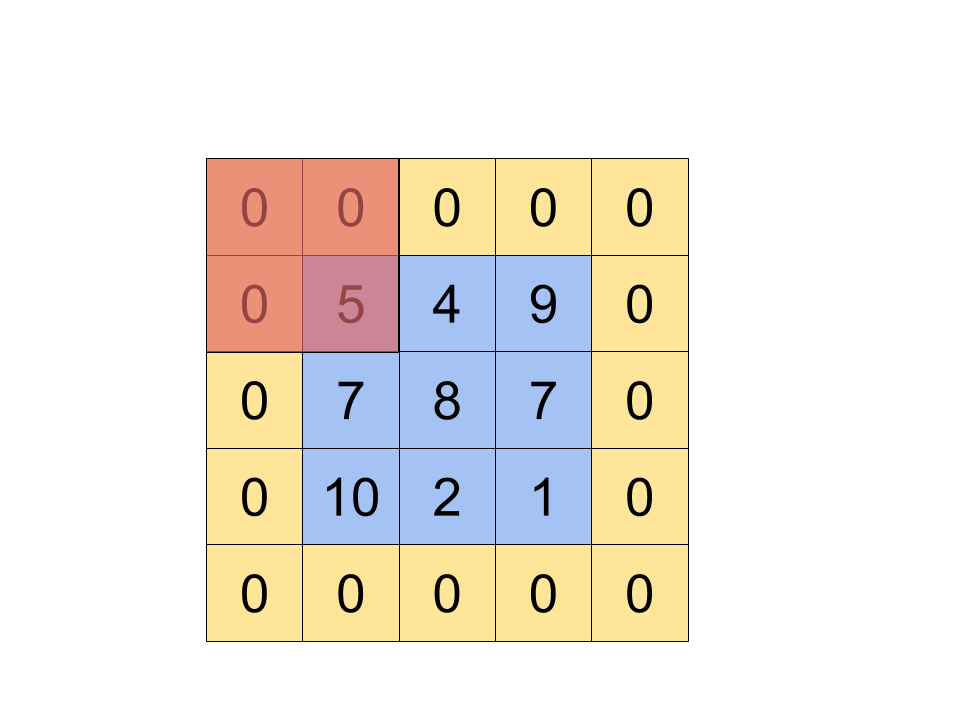
\includegraphics[width=.49\textwidth]{figs/ConvolutionExample.png}
\end{center}
\begin{small}
Figure: A convolution being applied to a $2 \times 2$ patch (the red square) of a $3 \times 3$ image that has been zero-padded to allow convolutions past the edges of the image.
\end{small}

What is one benefit and one drawback to this zero-padding scheme (in contrast to an approach in which we only perform convolutions over patches entirely contained within an image)?

\begin{solution}

No Padding : The output shrinks to (20-8+1) x (20-8+1) = 13 x 13
With Padding : The output remains 20 x 20

Benefit: With zero-padding we preserve the spatial dimensions of the output feature map. 
Witouth padding, the output shings from 20x20 to 13x13,
losing 7 pixels on each axis per layer. Over multiple comvolution layers,
this compounds and the spatial resolution collapses quickly. 

Drawback: With zero-padding we introduce artificial values, zeros, that do not correspond
to real image content. Convolutions computer near the vorders are therefores
operating over a mixture of real pixel data and fabricated zeros, which can 
produce lower quality or misleading features at the edges. Therefore,
the network may learn to detect patterns that are partly artifacts 
of the padding rather than meaningful image features.


\end{solution}

\newpage


\subsection{5 x 5 Convolutions}
Consider a single convolutional layer, where your input is a $32 \times 32$ pixel, RGB image. In other words, the input is a $32 \times 32 \times 3$ tensor. Your convolution has:

\begin{itemize}
\item Size: $5 \times 5 \times 3$
\item Filters: 8
\item Stride: 1
\item No zero-padding
\end{itemize}

\problem[2] What is the number of parameters (weights) in this layer, including a bias term?

\begin{subsolution}

We have 5 x 5 x 3 = 75 weights per filter, 1 bias term per filter, and 8 filters.
Total parameters = 8 x (75 + 1) = 608

\end{subsolution}

\newpage


\problem[3] What is the shape of the output tensor?

\begin{subsolution}
we need to calculate the output height and width using the formula:
Output Size = (Input Size - Filter Size) / Stride + 1
Output Height = (32 - 5) / 1 + 1 = 28
Output Width = (32 - 5) / 1 + 1 = 28
Output Depth = Number of Filters = 8
So the output tensor shape is (28, 28, 8)


\end{subsolution}

\newpage


 \subsection{Max/Average Pooling}
Pooling is a downsampling technique for reducing the dimensionality of a layer's output. Pooling iterates across patches of an image similarly to a convolution, but pooling and convolutional layers compute their outputs differently: given a pooling layer $B$ with preceding layer $A$, the output of $B$ is some function (such as the max or average functions) applied to patches of $A$'s output.

Below is an example of max-pooling on a 2-D input space with a $2\times 2$ filter (the max function is applied to $2\times 2$ patches of the input) and a stride of 2 (so that the sampled patches do not overlap):

\begin{center}
  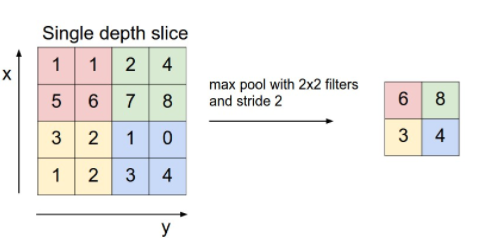
\includegraphics[width=.49\textwidth]{figs/MaxPool.png}
\end{center}

Average pooling is similar except that you would take the average of each patch as its output instead of the maximum.

Consider the following 4 matrices:
$$
\begin{bmatrix}
    1 & 1 & 1 & 0 \\
    1 & 1 & 1 & 0 \\
    1 & 1 & 1 & 0 \\
    0 & 0 & 0 & 0
\end{bmatrix},
%
\begin{bmatrix}
    0 & 1 & 1 & 1 \\
    0 & 1 & 1 & 1 \\
    0 & 1 & 1 & 1 \\
    0 & 0 & 0 & 0
\end{bmatrix},
%
\begin{bmatrix}
	0 & 0 & 0 & 0 \\
    0 & 1 & 1 & 1 \\
    0 & 1 & 1 & 1 \\
    0 & 1 & 1 & 1
\end{bmatrix},
%
\begin{bmatrix}
    0 & 0 & 0 & 0 \\
    1 & 1 & 1 & 0 \\
    1 & 1 & 1 & 0 \\
    1 & 1 & 1 & 0
\end{bmatrix}
$$
\problem[3]

Apply $2 \times 2$ average pooling with a stride of 2 to each of the above images.

\begin{subsolution}

\textbf{Matrix 1:}
$$\begin{bmatrix} 1 & 0.5 \\ 0.5 & 0.25 \end{bmatrix}$$
$$\begin{bmatrix} 0.5 & 1 \\ 0.25 & 0.5 \end{bmatrix}$$
$$\begin{bmatrix} 0.25 & 0.5 \\ 0.5 & 1 \end{bmatrix}$$
$$\begin{bmatrix} 0.5 & 0.25 \\ 1 & 0.5 \end{bmatrix}$$


\end{subsolution}

\newpage


\problem[3]

Apply $2 \times 2$ max pooling with a stride of 2 to each of the above images.

\begin{subsolution}
$$\begin{bmatrix} 1 & 1 \\ 1 & 1 \end{bmatrix}$$
$$\begin{bmatrix} 1 & 1 \\ 1 & 1 \end{bmatrix}$$
$$\begin{bmatrix} 1 & 1 \\ 1 & 1 \end{bmatrix}$$
$$\begin{bmatrix} 1 & 1 \\ 1 & 1 \end{bmatrix}$$
\end{subsolution}

\newpage


\problem[4]

Consider a scenario in which we wish to classify a dataset of images of various animals, taken at various angles/locations and containing small amounts of noise (e.g. some pixels may be missing). Why might pooling be advantageous given these distortions in our dataset?

\begin{subsolution}
In this case, pooling is advantageous because it provides spatial invariance and 
robustness to noise. 

If we apply 2x2 average pooling, we summarize a local region into a single value,
this means that if an animal shifts slightly in the frame, lets say a 
cat appearsa few pixels to the left in one image versus another, the poooled
output remain largely unchanged. This is translation invariance. 
For noise robustness, if some pixels are missing or corrupted,
ther max operation simply selects the strongest activation in the region,
ignoring the noise.
Additionally, pooling progressively reduces the spatial dimensions of the data,
which forces the network to focus on higher-level features(shapes, textures, body parts)
rather than exact pixel positions. This abstraction helps the model generalize better
to new images of animals taken from different angles. 
\end{subsolution}

\newpage


\subsection{PyTorch implementation}
\problem[20]

Using PyTorch ``Sequential'' model class as you did in 2C, build a deep \emph{convolutional}
network to classify the handwritten digits in MNIST. You are now allowed to use
the following layers (but \textbf{only} the following):

 \begin{itemize}
  \item \textbf{Linear:} A fully-connected layer
  \begin{itemize}
    \item In convolutional networks, Linear (also called dense) layers are typically used to knit together higher-level feature representations.
    \item Particularly useful to map the 2D features resulting from the last convolutional layer to categories for classification (like the 1000 categories of ImageNet or the 10 categories of MNIST).
    \item Inefficient use of parameters and often overkill: for $A$ input activations and $B$ output activations, number of parameters needed scales as $O(AB)$.
  \end{itemize}
  \item \textbf{Conv2d:} A 2-dimensional convolutional layer
  \begin{itemize}
    \item The bread and butter of convolutional networks, conv layers impose a translational-invariance prior on a fully-connected network. By sliding filters across the image to form another image, conv layers perform ``coarse-graining'' of the image.
    \item Networking several convolutional layers in succession helps the convolutional network knit together more abstract representations of the input. As you go higher in a convolutional network, activations represent pixels, then edges, colors, and finally objects.
    \item More efficient use of parameters. For $N$ filters of $K \times K$ size on an input of size $L \times L$, the number of parameters needed scales as $O(N K^2)$. When $N, K$ are small, this can often beat the $O(L^4)$ scaling of a Linear layer applied to the $L^2$ pixels in the image.

  \end{itemize}
  \item \textbf{MaxPool2d:} A 2-dimensional max-pooling layer
  \begin{itemize}
    \item Another way of performing ``coarse-graining'' of images, max-pool layers are another way of ignoring finer-grained details by only considering maximum activations over small patches of the input.
    \item Drastically reduces the input size. Useful for reducing the number of parameters in your model.
    \item Typically used immediately following a series of convolutional-activation layers.
  \end{itemize}
  \item \textbf{BatchNorm2d:} Performs batch normalization (Ioffe and Szegedy, 2014). Normalizes the activations of previous layer to standard normal (mean 0, standard deviation 1).
  \begin{itemize}
    \item Accelerates convergence and improves performance of model, especially when saturating nonlinearities (sigmoid) are used.
    \item Makes model less sensitive to higher learning rates and initialization, and also acts as a form of regularization.
    \item Typically used immediately before nonlinearity (Activation) layers.
  \end{itemize}
  \item \textbf{Dropout:} Takes some probability and at every iteration sets weights to zero at random with that probability
  \begin{itemize}
    \item An effective form of regularization. During training, randomly selecting activations to shut off forces network to build in redundancies in the feature representation, so it does not rely on any single activation to perform classification.
  \end{itemize}
  \item \textbf{ReLU (activation):} Sets negative inputs to 0
  \item \textbf{Softmax (activation):} Rescales input so that it can be interpreted as a (discrete) probability distribution.
  \item \textbf{Flatten:} Flattens any tensor into a single vector (required in order to pass a 2D tensor output from a convolutional layer as input into Linear layers)
\end{itemize}

\textbf{Your tasks.} Build a network with only the allowed layers that achieves \textbf{test accuracy of at least 0.985}. You are required to use categorical cross entropy as your loss function and to train for 10 epochs with a batch size of 32. Note: your model must have fewer than 1 million parameters, as measured by the method given in the sample code.
Everything else can change: optimizer (RMSProp, Adam, ???), initial learning rates, dropout probabilities, layerwise regularizer strengths, etc. You are not required to use all of the layers, but \emph{you must have
at least one dropout layer and one batch normalization layer in your final model}. Try to figure out the best possible architecture and hyperparameters given these building blocks!

In order to design your model, you should train your model for 1 epoch (batch size 32) and look at the final \textbf{test accuracy}  after training. This should take no more than 10 minutes, and should give you an immediate sense for how fast your network converges and how good it is.

Set the probabilities of your
dropout layers to 10 equally-spaced values $p \in [0, 1]$, train for 1 epoch, and report the final model accuracies for each.

You can perform all of your hyperparameter validation in this way: vary your parameters and train for an epoch. After you're satisfied with the model design, you should train your model for the full 10 epochs.

\textbf{In your submission.} Turn in the code of your model, the test accuracy for the 10 dropout probabilities $p \in [0, 1]$, and the
final test accuracy when your model
is trained for 10 epochs. We should have everything needed to reproduce your results.

Discuss what you found to be the most effective strategies in designing a convolutional network. Which regularization method was most effective (dropout, layerwise regularization, batch norm)?

Do you foresee any problem with this way of validating our hyperparameters? If so, why?

\emph{Hints:}

\begin{itemize}
	\item You are provided with a sample network that achieves a high accuracy. Starting with this network, modify some of the regularization parameters (layerwise regularization strength, dropout probabilities) to see if you can maximize the test accuracy. You can also add layers or modify layers (e.g.
	changing the convolutional kernel sizes, number of filters, stride, dilation, etc.) so long as the total number of parameters remains under the cap of 1 million.
  \item You may want to read up on successful convolutional architectures, and emulate some of their design principles. Please cite any idea you use that is not your own.
  \item To better understand the function of each layer, check the PyTorch documentation.
  \item Linear layers take in single vector inputs (ex: \emph{(784, )}) but Conv2D layers
	take in tensor inputs (ex: \emph{(28, 28, 1)}): width, height, and channels. Using the transformation \verb$transforms.ToTensor()$ when loading the dataset will reshape the training/test $X$ to a 4-dimensional tensor (ex: \emph{(num_examples, width, height, channels)}) and normalize values. For the MNIST dataset, \emph{channels=1}. Typical color images have 3 color channels, 1 for each color in RGB.
	\item If your model is running slowly on your CPU, try making each layer smaller
	and stacking more layers so you can leverage deeper representations.
	\item Other useful CNN design principles:
  \begin{itemize}
    \item CNNs perform well with many stacked convolutional layers, which develop increasingly large-scale representations of the input image.
    \item Dropout ensures that the learned representations are robust to some amount of noise.
    \item Batch norm is done after a convolutional or dense layer and immediately prior to an activation/nonlinearity layer.
    \item Max-pooling is typically done after a series of convolutions, in order to gradually reduce the size of the representation.
    \item Finally, the learned representation is passed into a dense layer (or two), and then filtered down to the final softmax layer.
  \end{itemize}
\end{itemize}

\begin{subsolution}
The most effective strategy was incorporating batch normalization 
after every convolutional layer, which stabilized and accelerated training.
BatchNorm stabilized training dramatically, allowing the model to reach 
98.7\% validation accuracy after just a single epoch.

I inmcreased the model capacity. Going from 8 filters per layer to 32 and 64
filters, and using two convolutional layers per block instead of one,
gave the network enough representational power to achieve high accuracy.
The model remained under 1 millon parameters limited at approximatly 470k paraneters, 

Dropout played a minor supporting role — the sweep showed
that low dropout values $(p = 0.0 to 0.4)$ all performed 
similarly well, while high values $(p \geq 0.889)$ produced bad results,
collapsing accuracy to random chance ($\sim$10--13\%).

Do I foresee any problem with this way of validating our hyperparameters? 
The main problem is related to the dopout selection process itself. When we trainined 
10 models with different dropout probabilities for a single epoch each,and
choosing the one that performed bes on the test set, we leaked
information from the test set into our model selection process.
This means the reported test accuracy is an optimistically biased 
estimate of true generalization performance, because our design 
decisions were influenced by test set results. In this case it would have been better
k-fold cross-validation on the training set for hyperparameter 
tuning, and reserve the test set exclusively for a single final evaluation. 



\end{subsolution}

\begin{table}[h!]
\centering
\caption{Test accuracy after 1 epoch for different dropout probabilities}
\begin{tabular}{c c}
\hline
Dropout $p$ & Test Accuracy \\
\hline
0.000 & 0.9918 \\
0.111 & 0.9909 \\
0.222 & 0.9878 \\
0.333 & 0.9902 \\
0.444 & 0.9894 \\
0.556 & 0.9874 \\
0.667 & 0.9811 \\
0.778 & 0.9750 \\
0.889 & 0.1243 \\
1.000 & 0.1328 \\
\hline
\end{tabular}
\label{tab:dropout_sweep}
\end{table}

\newpage

\begin{lstlisting}[language=Python]
  import torch.nn as nn

class MyModel(nn.Module):
    def __init__(self, dropout_p=0.3):
        super().__init__()
        self.net = nn.Sequential(
            # Block 1
            nn.Conv2d(1, 32, 3, padding=1),
            nn.BatchNorm2d(32),             
            nn.ReLU(),
            nn.Conv2d(32, 32, 3, padding=1),
            nn.BatchNorm2d(32),
            nn.ReLU(),
            nn.MaxPool2d(2),
            nn.Dropout(dropout_p),           

            # Block 2
            nn.Conv2d(32, 64, 3, padding=1),
            nn.BatchNorm2d(64),
            nn.ReLU(),
            nn.Conv2d(64, 64, 3, padding=1),
            nn.BatchNorm2d(64),
            nn.ReLU(),
            nn.MaxPool2d(2),
            nn.Dropout(dropout_p),

            # Classifier
            nn.Flatten(),
            nn.Linear(64 * 7 * 7, 128),     
            nn.BatchNorm1d(128),
            nn.ReLU(),
            nn.Dropout(dropout_p),
            nn.Linear(128, 10)
        )

    def forward(self, x):
        return self.net(x)
\end{lstlisting}


\begin{lstlisting}[language=Python]
import numpy as np

device = torch.device('cuda' if torch.cuda.is_available() else 'cpu')
print(f"Using device: {device}")

dropout_results = {}

for p in np.linspace(0, 1, 10):
    model = MyModel(dropout_p=p).to(device)          
    optimizer = torch.optim.Adam(model.parameters(), lr=0.001)
    criterion = nn.CrossEntropyLoss()

    # train 1 epoch
    model.train()
    for i, data in enumerate(training_data_loader):
        images, labels = data
        images, labels = images.to(device), labels.to(device)  
        optimizer.zero_grad()
        output = model(images)
        loss = criterion(output, labels)
        loss.backward()
        optimizer.step()

    # evaluate
    model.eval()
    test_correct, test_total = 0, 0
    with torch.no_grad():
        for data in test_data_loader:
            images, labels = data
            images, labels = images.to(device), labels.to(device) 
            output = model(images)
            _, predicted = torch.max(output.data, 1)
            test_total += labels.size(0)
            test_correct += (predicted == labels).sum().item()

    acc = test_correct / test_total
    dropout_results[p] = acc
    print(f"p={p:.3f} --> Test Acc: {acc:.4f}")

print("\n--- Results ---")
for p, acc in dropout_results.items():
    print(f"p={p:.3f}: {acc:.4f}")

\end{lstlisting}

\begin{lstlisting}[language=Python]
# Train the model for 10 epochs, iterating on the data in batches
n_epochs = 10

device = torch.device('cuda' if torch.cuda.is_available() else 'cpu')
model = MyModel(dropout_p=0.111).to(device)
optimizer = torch.optim.Adam(model.parameters(), lr=0.001)  
criterion = nn.CrossEntropyLoss()                            

# store metrics
training_accuracy_history = np.zeros([n_epochs, 1])
training_loss_history = np.zeros([n_epochs, 1])
validation_accuracy_history = np.zeros([n_epochs, 1])
validation_loss_history = np.zeros([n_epochs, 1])

for epoch in range(n_epochs):
    print(f'Epoch {epoch+1}/10:', end='')
    train_total = 0
    train_correct = 0
    # train
    model.train()
    for i, data in enumerate(training_data_loader):
        images, labels = data
        images, labels = images.to(device), labels.to(device)  
        optimizer.zero_grad()
        # forward pass
        output = model(images)
        # calculate categorical cross entropy loss
        loss = criterion(output, labels)
        # backward pass
        loss.backward()
        optimizer.step()

        # track training accuracy
        _, predicted = torch.max(output.data, 1)
        train_total += labels.size(0)
        train_correct += (predicted == labels).sum().item()
        # track training loss
        training_loss_history[epoch] += loss.item()
        # progress update after 180 batches (~1/10 epoch for batch size 32)
        if i % 180 == 0: print('.',end='')
    training_loss_history[epoch] /= len(training_data_loader)
    training_accuracy_history[epoch] = train_correct / train_total
    print(f'\n\tloss: {training_loss_history[epoch,0]:0.4f}, acc: {training_accuracy_history[epoch,0]:0.4f}',end='')

    # validate
    test_total = 0
    test_correct = 0
    with torch.no_grad():
        model.eval()
        for i, data in enumerate(test_data_loader):
            images, labels = data
            images, labels = images.to(device), labels.to(device)  # <-- added
            # forward pass
            output = model(images)
            # find accuracy
            _, predicted = torch.max(output.data, 1)
            test_total += labels.size(0)
            test_correct += (predicted == labels).sum().item()
            # find loss
            loss = criterion(output, labels)
            validation_loss_history[epoch] += loss.item()
        validation_loss_history[epoch] /= len(test_data_loader)
        validation_accuracy_history[epoch] = test_correct / test_total
    print(f', val loss: {validation_loss_history[epoch,0]:0.4f}, val acc: {validation_accuracy_history[epoch,0]:0.4f}')

\end{lstlisting}

\end{document}
